\chapter{理论模型}
\section{利用词嵌入技术构造新型元数据}
\subsection{文件名、目录名的向量化}
在Unix文件系统中,任意文件或目录在被创建时,均会被分配一个唯一的ID,也就是Inode序号,以此作为唯一的标识以便于后续各种文件操作。Inode序号只与文件创建先后相关,是一种one-hot的表示方式。那么能否效仿自然语言处理中词嵌入的思想,建立一种能够包含文件或目录之间关联性的表征方式?

文件系统层次结构规范(Filesystem Hierarchy Standard,FHS)\cite{fhs}是由Linux基金会在1994年发起,旨在规范Linux各发行版和其他类Unix系统下文件目录结构的业界统一标准,至今已发展演变到FHS-3.0(2015年)。在FHS定义的目录结构规范下,Linux操作系统的目录组织结构和命名受到了明确严格的约束,例如:
\begin{itemize}
    \item /:根目录。
    \item /bin:系统执行文件目录。
    \item /boot:启动文件目录。
    \item /dev:驱动设备目录。
    \item /etc:系统配置文件目录。
    \item /lib, /usr/lib, /usr/local/lib:系统使用的函数库目录。
    \item ......
\end{itemize}

如果将一个文件的完整路径(如/usr/lib/python2.7/)视为一个句子,各级目录视为单词,我们假定上节提到的分布式假设同样成立,即:同一目录下的文件或目录具有类似的含义。直观上看,这个假设是合理的,例如/bin目录下的bash,rm,cp文件等均为可执行命令,/usr/lib/python2.7/目录下均为Python的库文件。在此假设成立的前提下,本节将介绍如何使用Skip-gram模型,对给定的Unix文件系统目录下所有文件名、目录名进行向量化。

\subsubsection*{语料库的生成}
众所周知,任何机器学习模型都离不开数据,自然语言处理领域的数据集通常被称为语料库(Corpus)。任何语言学的研究或者自然语言模型的建立都必须建立在大量的语料之上,否则无论是基于规则方法还是统计方法建立的模型都将失效。

为了建立文件路径相关的“语料库”,我们将从根目录(或文件系统的挂载点)开始,通过常规的遍历算法将此目录下所有文件、目录的完整路径逐行写入到一个文本文件,作为模型的训练数据集。语料库生成后,相应地可以得到一个词汇表$V$。
{\color{red}此处插入遍历算法}

\subsubsection*{利用Skip-gram模型训练文件和目录名的词向量}
给定总单词数量为$T$的语料库,其词汇表$\mathcal{V}$=\{\textit{bin,boot,dev,...}\},词汇数量为$W$。
%其中任意一个词可用其在词汇表中的序号表示:$w \in \{1,\dots,W\}$。
那么该语料库可表示为一个由$T$个词向量组成的序列:$\mathbf{w}_1, \mathbf{w}_2, \dots, \mathbf{w}_T$。Skip-gram模型的目标就是建立一个从词汇表到$d$维向量空间的映射$model:\mathcal{V} \rightarrow \mathbb{R}^d$,使以下对数极大似然函数达到最大:
\begin{equation}
    \label{eq:origin_object}
    \frac{1}{T}\sum_{t=1}^T \sum_{c \in \mathcal{C}_t} \log p(\mathbf{w}_c | \mathbf{w}_t),
\end{equation}

其中,$\mathcal{C_t}$表示某中心词$\mathcal{w}_t$的上下文中出现过的词的集合。以路径\textit{/usr/local/lib/python}为例,若取上下文窗口大小为1,那么中心词$\mathcal{w}_t$=\textit{lib}的上下文集合$\mathcal{C_t}$=\{\textit{local,python}\}。对于任意样本$(\mathbf{\mathcal{w}}_t,\mathbf{\mathcal{w}}_c)$,我们用归一化函数softmax来定义单词$\mathcal{w}_c$在中心词$\mathbf{\mathcal{w}}_t$的上下文中出现的条件概率:
\begin{equation}
    \label{eq:softmax}
    p(\mathbf{w}_c | \mathbf{w}_t)=\frac{ e^{ \mathbf{w}_t^{\top} \mathbf{w}_c} }{ \sum_{j=1}^W e^{\mathbf{w}_t^{\top} \mathbf{w}_j}} 
\end{equation}

\begin{figure}[htp]
\centering
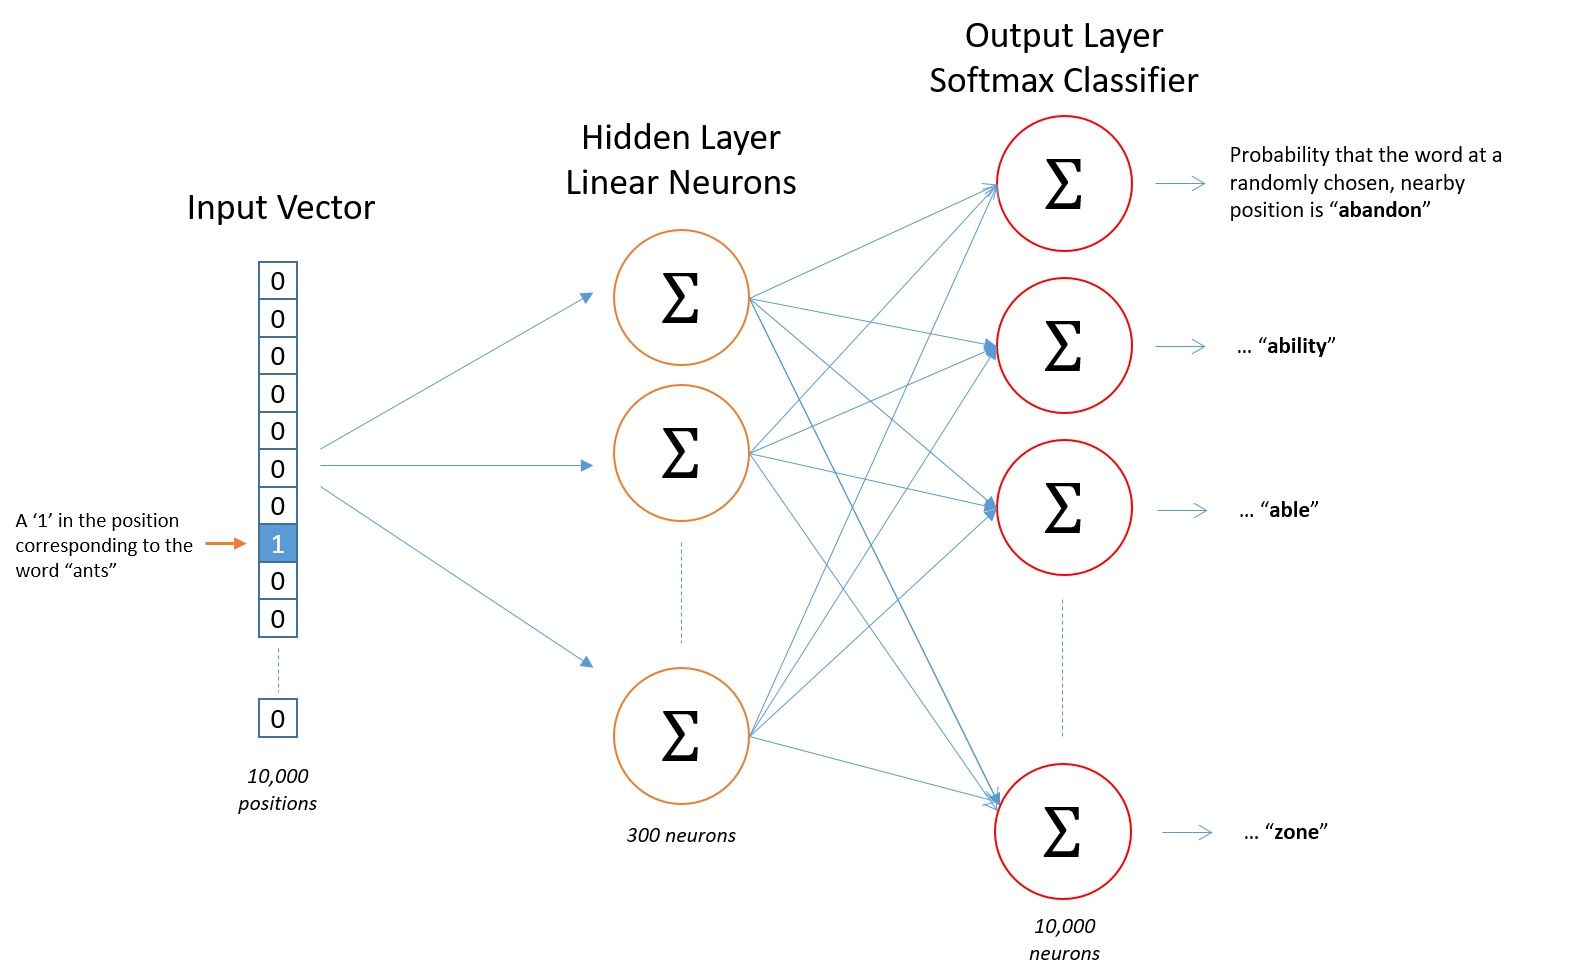
\includegraphics[width=\textwidth]{word2vec_nn}
\caption{Skip-gram模型网络}
\label{fig:word2vec_nn}
\end{figure}
如图\ref{fig:word2vec_nn},Skip-gram模型是一个三层神经网络,输入为词汇表中单词的初始向量,即$W$维的one-hot编码。隐层由$d$个神经元组成,没有激活函数,只有权值。训练收敛后隐层的$W\times d$的权值矩阵就是词汇表内所有词向量的集合。输出层为上文所述的softmax函数,最终结果是一个$W$维的向量,每个分量表示对应的单词与输入词存在上下文关系的概率。

当语料库规模较大,词汇表内单词较多时,采用softmax函数的计算复杂度过高。一种优化方式是使用层次化softmax(Hierarchical softmax)\cite{Hierarchical_softmax}。另一种计算复杂度更低,且同样能保证对原有softmax层拟合精度的优化方式是负采样(Negative sampling),
%噪声对比估计(Noise Contrastive Estimation,NCE),也称为,
一种用来提高训练速度且能改善词向量质量的方法。该方法将中心词上下文中的单词视为正类样本,并在词汇表中随机抽取若干(通常取5至20个)非上下文的噪声词作为负样本,对公式\ref{eq:softmax}中的softmax函数作了如下拟合:
\begin{equation}
    \label{eq:neg}
    \log(1+e^{-\mathbf{w}_t^{\top} \mathbf{w}_c})+ \sum_{n \in \mathcal{N}_{t,c} }\log(1+ e^{\mathbf{w}_t^{\top} \mathbf{w}_n})
\end{equation}
其中$\mathcal{N}_{t,c}$表示词汇表出去中心词t和上下文c之后,随机抽取的若干噪声词组成的负样本集合。

用sigmoid函数$\sigma:x \rightarrow \log(1+e^{-x})$与公式\ref{eq:neg}代入目标函数\ref{eq:origin_object}得到最终的目标函数:
\begin{equation}
    \frac{1}{T} \sum_{t=1}^{T} \left[ \sum_{c \in \mathcal{C}_t} \sigma(\mathbf{w}_t^{\top} \mathbf{w}_c) + \sum_{n \in \mathcal{N}_{t,c}} \sigma(-\mathbf{w}_t^{\top} \mathbf{w}_n) \right]
\end{equation}

经过以上优化后,Skip-gram模型训练的计算复杂度大大缩小。隐层的$W\times d$的权值矩阵通过随机梯度下降训练收敛后,作为最终词汇表$\mathcal{V}$的词向量模型。

\subsection{引入子词模型}
%阐述文件系统内命名与人类自然语言的区别,与前文FastText中的子词模型呼应
\subsection{路径向量}
%注意区分绝对路径、工作路径、挂载点等造成的差异
\section{基于门控神经网络的热点数据识别}
\subsection{问题定义}
设文件系统进行文件向量化处理后,所有文件向量($d$维)组成的集合记为$\mathcal{F} \subset \mathbb{R}^d$。在某工作负载的生命周期内对其文件访问进行追踪,将追踪日志转化为$d$维路径向量序列$\mathcal{S}=\{\mathbf{x}_1, \mathbf{x}_2,\dots, \mathbf{x}_T\}$。
设上下文窗口大小为$N$,即
在任意时刻$t$,追踪模块对前$N$次访问构成的子序列$\{\mathbf{x}_{t-N+1}, \dots, \mathbf{x}_t\}$记为$\mathcal{S_t}$。
定义该时刻的上下文序列$\mathcal{S}_c = \{ \mathbf{x}_{t-N+1}, \dots, \mathbf{x}_{t+N} \}$为正类样本,其余所有文件$\mathcal{F} - \mathcal{S}_c$为负样本(冷文件)。

建立模型$M$,以$\mathcal{S}_t$为输入计算这段访问序列所隐含的访问模式$h$(也是一个$d$维向量)。同时定义分类函数$f:\mathbb{R}^d \times \mathcal{F} \rightarrow \{0,1\}$,对任意文件$\mathbf{x} \in \mathcal{F}$,当$f(h,\mathbf{x})=1$时判定其为热文件,否则为冷文件。
\subsection{基于门控神经网络的模型设计}


%指标以命中率、错判率为主,即准确率召回率?
\section{本章小结}